\documentclass[a4paper]{article}

%% Language and font encodings
\usepackage[english]{babel}
\usepackage[utf8x]{inputenc}
\usepackage[T1]{fontenc}

%% Sets page size and margins
\usepackage[a4paper,top=3cm,bottom=2cm,left=3cm,right=3cm,marginparwidth=1.75cm]{geometry}
\linespread{1.25}
%% Useful packages
\usepackage{amsmath}
\usepackage{graphicx}
\usepackage{subcaption}
\usepackage[colorinlistoftodos]{todonotes}
\usepackage[colorlinks=true, allcolors=blue]{hyperref}


\graphicspath{ {./figs} }

\begin{document} %{{{

\title{Novelty, Familiarity, and the Success of Fanfictions among Fans} %{{{
\date{\today}
\maketitle %}}}

What do the fans like? The creative industries, an economic sector that generates billions of dollars of output every year in the U.S. with cultural products such as movies, TV shows and video games \cite{creativeindustries}, are constantly trying to solve this puzzle. On the one hand, novelty or innovation is central to creative works, and people seek surprise when consuming such products \cite{hutter2011infinite}; and on the other hand, psychological evidences have shown that people also have a strong preference for familiarity. For example, mere exposure can increase people's preference for a stimuli \cite{zajonc1968attitudinal}, even when they are not aware of the exposure \cite{kunst1980affective}. The exposure effect is assumed to have an evolutionary basis, and has been verified by multiple experiments \cite{bornstein1989exposure}.

Providing fans with things they are familiar with can therefore be used as a strategy to increase affinity. Repetition has long been utilized in cultural products including music and poetry \cite{huron2013psychological}. This trend can be also found in the contemporary popular culture, where many new releases are adaptations, remakes, and ``remixes'' \cite{manovich2007comes} of existing works. For example, in the movie industry, the companies Marvel and DC have been making movies based on their popular comics, including many sequels, prequels and ``reboots''. In an extreme case, the origin story of the Spider-man has been re-played in three movies since 2002 \cite{spiderman}. Market reception indicates that the audience welcome these products: out of the 10 highest-grossing movies of 2016, 8 are adaptions, sequels, remakes, or part of a movie universe \cite{2016film}. This number increased to 10 out of 10 in 2017 \cite{2017film}. 

To reconcile the seeming conflict between the preference for novelty and familiarity, the optimal differentiation hypothesis has been widely adopted. It states that successful creative works are combinations of convention and innovation: the most popular ones are differentiated from previous works and their peers, but not \emph{too} different. In psychology, this is captured in the Wundt-Berlyne curve, which suggests that when exposed to novel stimuli, a perceiver's positive feelings first increase as novelty increases, until reaching a certain threshold; afterwards, further increasing novelty will lead to a decrease in positive feelings \cite{berlyne1970novelty}. Experiments have supported this hypothesis \cite{hargreaves1984effects} \cite{sluckin1980liking}, and it has been used to study the success of a variety of cultural products. For example, Askin and Mauskapf has found that songs with optimal differentiation are more likely to be on the top of the Billboad's Hot 100 charts \cite{askin2017makes}. Sreenivasan found a similar pattern for films \cite{sreenivasan2013quantitative}, and Mukherjee et al. found that in scientific publications, the highest-cited papers are grounded on mostly conventional, but partly novel combinations of previous works. 

However, most of these researches rely on external metrics to measure the success of creative works, such as the box office or the positions on the Billboard chart. These are highly influenced by factors not directly relevant to a creative works' quality, such as advertisement and media coverage. In particular, the consumers' choices are largely shaped by the herding behavior: for example, it was found that being on the New York Times bestseller list will cause an increase in a book's following sales \cite{sorensen2007bestseller}.  Even a ``faked'' popularity can be turned into real popularity as people are more likely to view creative works that they perceive to be popular \cite{salganik2008leading}. Therefore, such metrics may not accurately reflect the consumers' actual enjoyment of a cultural product. Moreover, as the features of cultural products vary significantly across genres, lengths, subjects, and more, it is hard to measure the novelty or conventionality of one piece against the others. 

We instead study a special type of creative works that are directly created and consumed by fans -- fan works. Known formally as transformative works, they are creative works made by fans based on one or more original works (``canons'') \cite{wiki:transf_work}. For example, a story written by a contemporary fan about Sherlock Holmes in his retirement is considered a fan work. Although fan works have multiple media types such as art, music and games, one of the most common type is creative writing: fanfictions. As a unique cultural phenomena, fanfictions have drawn attention from media studies and cultural studies \cite{thomas2011fanfiction}. However, most of the existing studies focus on the identity of fanfiction writers \cite{black2006language}, the practice of fanfiction writing \cite{LIT:LIT12061}, and the interaction between fans \cite{hills2015expertise}, and it is difficult to find studies that focus on fanfictions themselves as creative works.

Using fanfictions as subjects of study, we may avoid some of the complications mentioned above. The success of a fanfiction can be measured directly: in our dataset, readers can click ``Kudos'' to express that they enjoyed reading a fanfiction. As a subculture, fanfictions are usually not published as books nor featured in mainstream media, and there is no ``bestseller list'' for fanfictions, therefore fans usually discover and evaluate fanfictions more independantly. Additionally, most fanfictions are freely available in the Internet, so that the price will not be a confounding factor. Regarding the intrinsic features, fans of a canon usually form communities known as fandoms \cite{wiki:fandom}, and fanfictions in a fandom share a homogenous context, reducing the variation in subjects. More importantly, the well-developed text mining and natural language processing methods allow us to quantify the novelty of a fanfiction based on its linguistic features.

With these advantages, we investigate how a fanfiction's novelty or familiarity influences its success. We use three methods to quantify a fanfiction's novelty: one based on the word features, one on the topic features, and one based on its author-generated tags. A fanfiction is more novel if it has a large distance to other fanfictions published during the same time period in the feature space, and vice versa. Using statistical models, we found a negative relationship between a fanfiction's novelty and its success, consistent across our three metrics for novelty, suggesting that in disproval of the optimal differentiation hypothesis, fanfiction readers prefer familiarity and discourage novelty in general.


%Fandoms have developed into very large communities, especially in the Internet. The data source of our study, ArchiveOfOurOwn.org, is an online fanfiction archive that allows users to upload their fictions, and categorizes them based on fandoms. Established in 2009, it has 1,313,000 users and 3,423,000 pieces of fanfictions by November 2017 \cite{ao3stats}.

%The authors and readers' passion about fanfictions alludes to a balance between novelty and familiarity: they desire to see familiar characters and elements, but in novel stories. By analyzing people's perception of fanfictions, we may gain a better understanding of this balance. 

%Researches are only starting towards a quantitative definition of novelty. Many have employed a network approach, defining a creative work's novelty by looking at how they reference previous works \cite{elgammal2015quantifying}\cite{wang2013quantifying}\cite{2017arXiv170704239I}. In some cases, tags of a work can be used to evaluate its novelty\cite{sreenivasan2013quantitative}. 


%While the text of fanfictions directly capture their contents, the tags generated by authors (see Methods) provides a summary of the fictions. Authors often use tags to describe the genre and plot of their fictions, for example, ``Angst'' or ``Alternative Universe''. Although a user is free to use any tag, when she starts to enter a tag, the website will prompt with tag suggestions, avoiding multiple synonyms. The tag set of a fiction provides an abstraction of its content. Besides the language modeling approach, we also ran a separate analysis on the tag set.


%Story telling is one of human beings' basic needs and abilities\cite{gottschall2012storytelling}. Despite having endless forms, most stories can be considered as variations of one of the basic archetypes. In mythology studies, Campbell deduced a fundamental structure, \emph{the hero's journey}, from all major myths around the world \cite{campbell2008hero}. Levi-Strauss broke down different versions of a myth to identify common mythemes \cite{levi1955structural}. In oral legends and tales, many stories had a certain origin and developed into different versions through time and interaction between creators. Myths and folktales in oral traditions of civilizations around the world often follow this pattern, for example, the tale of the \emph{Little Red Riding Hood} originated approximately in the 10th century, and has developed multiple variations\cite{littlered}. Some elements of the legend \emph{Mahabharata} can be traced back to the Vedic period (15--6 century B.C.) as oral tales told by bards, and was textualized into many versions\cite{van2011mahabharata}.

%Thomas \cite{thomas2011fanfiction} summarizes the study of fanfictions into several main stages: Earliest researches characterized the fanfiction writers as "rebels" against the powerful authority of the original work. Later researches attempted to generate a deeper understanding to this simplified view, and started responding to the new media forms that facilitated fan activities and interactions. Some recent studies shifted their emphasis to the contributions of fans to contemporary culture. 

% Similar to other creative works, fanfictions are constantly under selection and evaluation from their readers. %The most successful fanfictions in the market have been published and even adapted into other media forms, accepted by the main stream (for example, \emph{Fifty Shades of Grey} was originally a fanfiction of \emph{Twilight}), while the majority of them remain mostly unknown.



\section*{Results} 
We first present some descriptive statistics of our data. 


\subsection*{Statistics of the fanfiction dataset}

Figure \ref{fig:fandom_size} shows the number of fictions in each of the 25 fandoms that we study. Our data collection includes fandoms in each of the broad categories based on medium: movies, TV shows, books, anime \& manga, and musicals (see Methods). The fandoms with the most fictions are \emph{Marvel}, \emph{Supernatural}, and \emph{Harry Potter}. Figure \ref{fig:fic_time_dist}  shows the time distribution of fictions published. As AO3 was established in December 2009, the fictions earlier than this time might be migrated from other platforms, thus may not correctly reflect the online community. We therefore only run our analysis using the fictions published in January 2010 and later. After the establishment, the site first experienced a slow growth until around 2012, when the number of fictions published begin to rise radically. At its peak in early 2016, more than 70,000 fictions were published in a month.


\begin{figure}
    \centering
    \begin{subfigure}[b]{0.7\textwidth}
        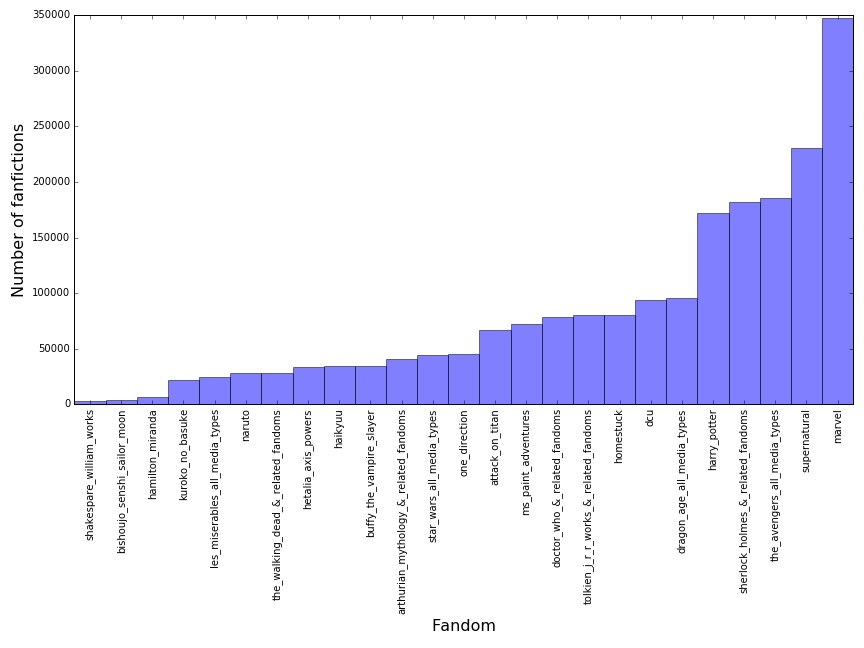
\includegraphics[width=\textwidth]{/fandom_size.png}
        \caption{Number of fanfictions in each fandom}
        \label{fig:fandom_size}
    \end{subfigure}
    ~ %add desired spacing between images, e. g. ~, \quad, \qquad, \hfill etc. 
      %(or a blank line to force the subfigure onto a new line)
    \begin{subfigure}[b]{0.7\textwidth}
        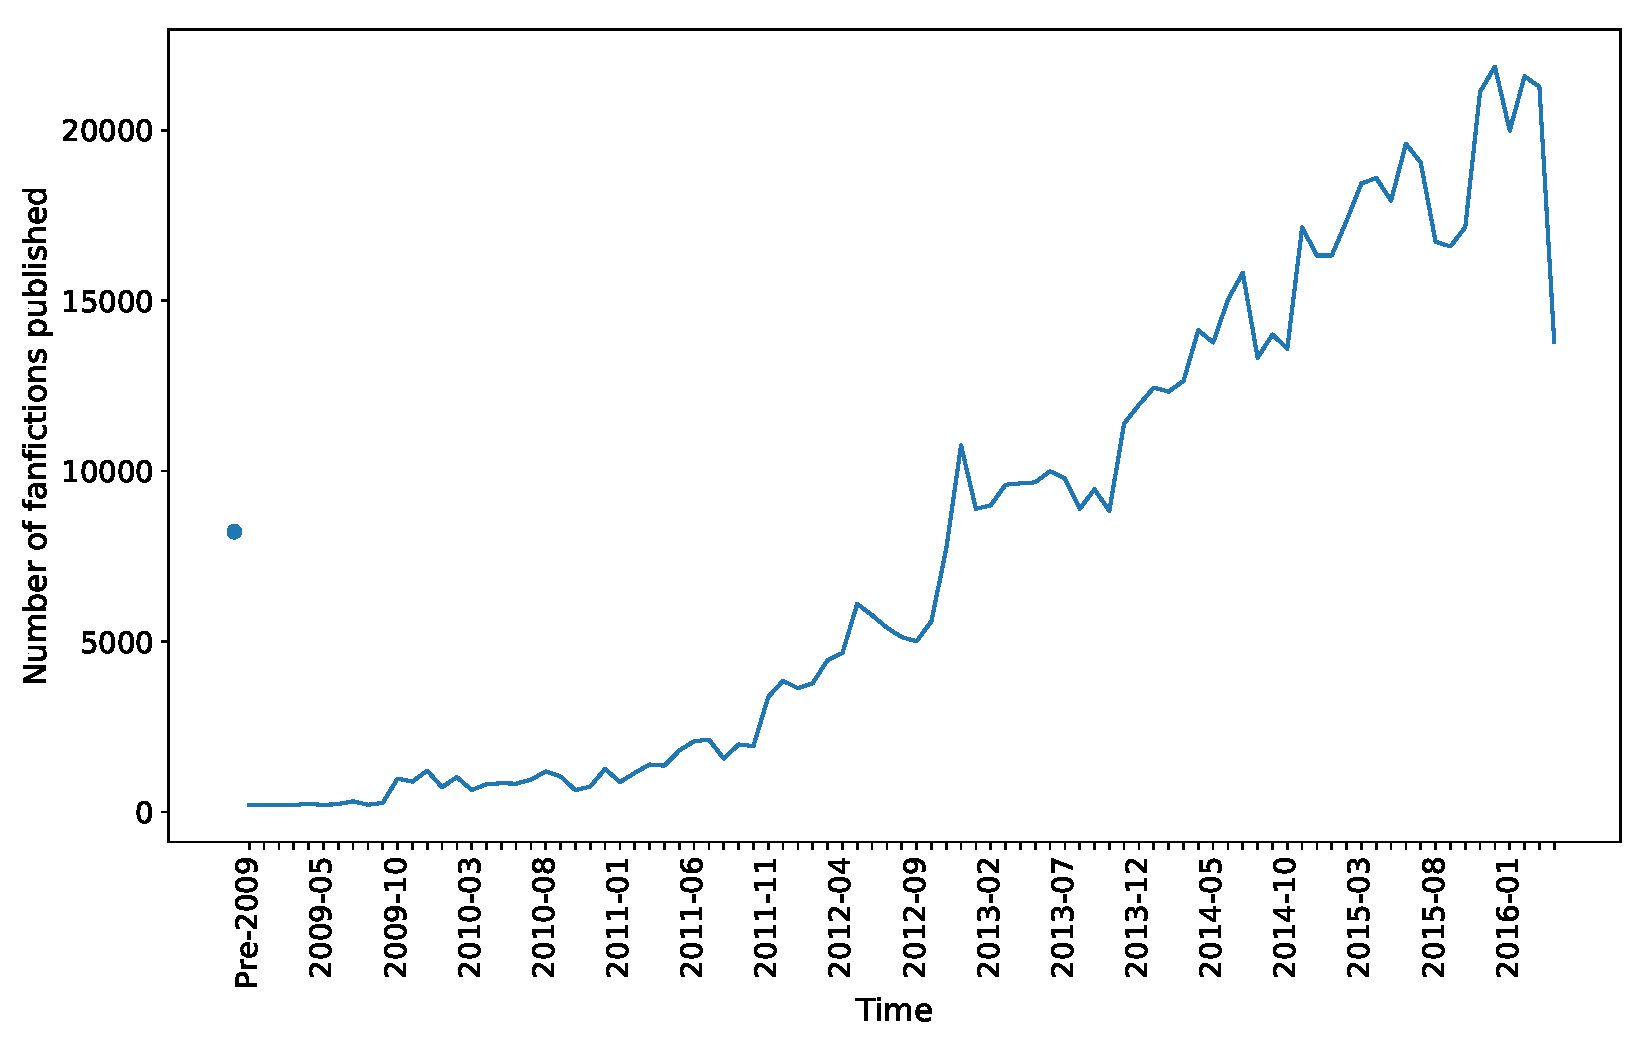
\includegraphics[width=\textwidth]{/fic_time_dist.pdf}
        \caption{Number of fanfictions published each month}
        \label{fig:fic_time_dist}
    \end{subfigure}
    \caption{Statistics of the size and temporal distribution of our fanfiction dataset}\label{fig:stats_size_time}
\end{figure}

The length distribution of the fanfictions is presented in Figure \ref{fig:length_dist} . Since many fictions have multiple chapters, we consider length as the average number of words in each chapter. A great variation of average length can be observed. The variation of length in documents can have a significant effect on the distance between documents, biasing towards shorter distance between longer documents. A similar issue has been noticed in vector space models very early on \cite{singhal2017pivoted}, where many normalization methods have been proposed to correct it. Instead of applying a normalization, in our analysis, we sample a fixed length (1,000 words) from each document. 

Figure \ref{fig:fic_time_dist} shows the logged cumulative distribution of Kudos. Following a long-tailed distribution, a small number of fictions receive the majority of Kudos, while most fictions receive little or no Kudos. Because of this pattern, we use the log of Kudos to evaluate the success of fictions. 

In Figure \ref{fig:tag_set_len}, we observe the tag set length of the fictions. The majority of fictions has under 20 tags, with a few having as many as 150 tags. Because the users have the liberty to create any tag, many of the tags will not be reused. To reduce the influence of infrequent tags, we therefore discard the tags that appear only once.

\begin{figure}
    \centering
    \begin{subfigure}[b]{0.7\textwidth}
        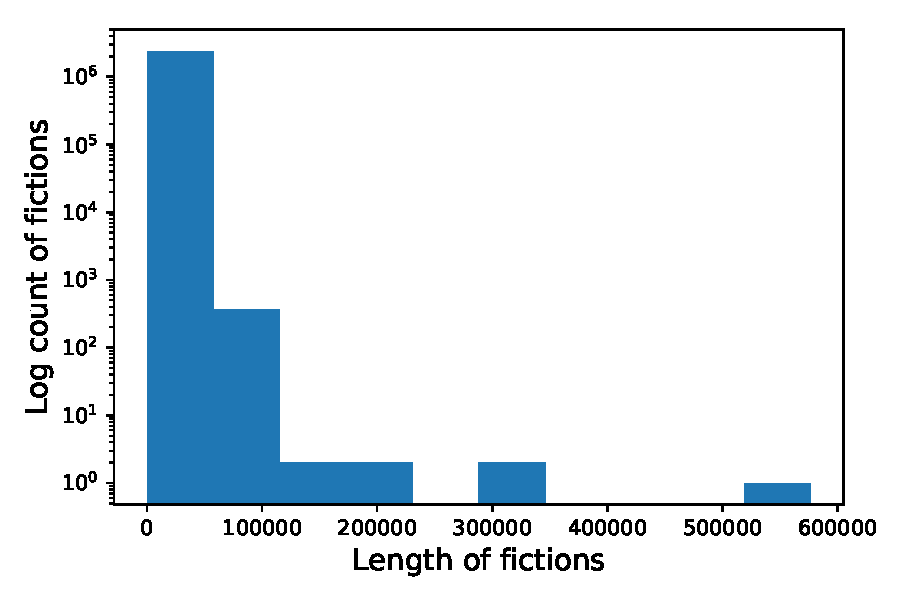
\includegraphics[width=\textwidth]{/fic_len_dist.pdf}
        \caption{Length distribution of fictions. For multi-chapter fictions, we show the average length of each chapter.}
        \label{fig:length_dist}
    \end{subfigure}
    ~ %add desired spacing between images, e. g. ~, \quad, \qquad, \hfill etc. 
      %(or a blank line to force the subfigure onto a new line)
    \begin{subfigure}[b]{0.7\textwidth}
        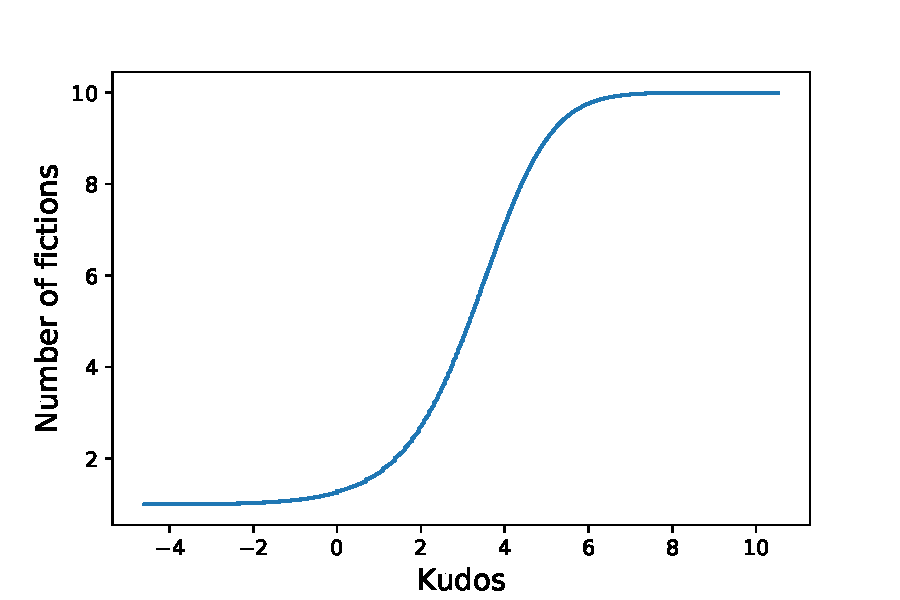
\includegraphics[width=\textwidth]{/kudos_dist.pdf}
        \caption{Linear-log cumulative distribution of Kudos. For multi-chapter fictions, we use the average number of Kudos per chapter. A long-tail distribution is observed, where a small portion of fictions receive the majority of Kudos.}
        \label{fig:kudos_dist}
    \end{subfigure}
    \caption{Statistics on the length and Kudos of fictions}\label{fig:stats_len_kudos_tags}

\end{figure}

\begin{figure}
    \centering
        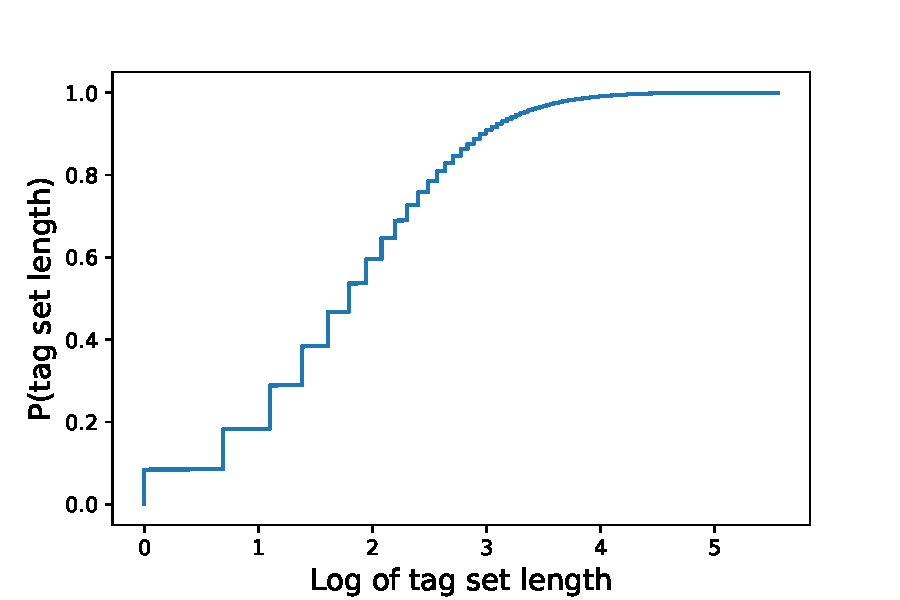
\includegraphics[width=0.7\textwidth]{/tag_len_dist.pdf}
        \caption{Linear-log cumulative distribution of tag set length. }
        \label{fig:tag_set_len}
\end{figure}

\subsection*{Document novelty and success}
We create two distinct measurements for the novelty of fanfiction documents, and employ them to identify the relationship between novelty and the number of Kudos that they receive. A negative correlation is observed, consistent across both measurements. Figure \ref{fig:unigram_cos} shows the result from the unigram language model. Under this model, a fixed number of words (1,000 in our experiment) is sampled from each document in a bag-of-words approach, where the ordering of words is not preserved. We then calculate the probability distribution over the unigrams. To account for unseen unigrams, we apply the Simple Good-Turing smoothing method \cite{gales1995good}, which assigns a small non-zero probability to those unigrams. 

The novelty score of each fiction is computed by comparing it to an ``average" fiction. To define the ``average" fiction, we take a set of fictions consisting of all fiction published within the past 6 months before the target fiction is published. Then we calculate the average probability distribution of the fictions in this set. We compute the novelty score of the fiction as the cosine distance between the target fiction and the average fiction:

\begin{equation}
n = 1-\frac{\sum_{i=1}^{n}{A_iB_i}}{\sqrt{\sum_{i=1}^{n}{A_i^2}}\sqrt{\sum_{i=1}^{n}{B_i^2}}}
\end{equation}

From Figure \ref{fig:unigram_cos}, we observe that as the novelty score increases between 0 and 1, the z-score of Kudos steadily decrease from 0.1 to -0.3: that is, from above average to below average. 

Besides the language model, we also present the results of running a topic modeling algorithm to detect the topics of fanfictions. 
The \emph{Latent Dirichlet Allocation} (LDA) \cite{blei2003latent} has been widely used for such tasks. As an unsupervised learning algorithm, it models a topic as a probabilistic distribution over a set of words, and a document as a probabilistic distribution over a set of topics. We are thus able to compute the distance between documents by comparing their topic compositions. Similar to the unigram model, we construct an ``average'' fiction as the average topic distribution of fictions in a set consisting of fictions published during a given time period, and define the novelty score as the cosine distance between a fiction and the average fiction. Figure \ref{fig:lda_cos} shows the results of the LDA model. Consistent with the result of the unigram model, as novelty scores increase, the z-score of Kudos decrease from positive (above average) to negative (below average).

\subsection*{Tag novelty and success}
We adapt the method from \cite{sreenivasan2013quantitative} to compute a novelty score for each tag. This method considers the ``surprise" of observing a tag, given a set of tags from all fictions in the past. To control for the size of the size of this set, we use a limited length of past history, only considering the fictions published within 6 months of the target fiction. First, we compute the probability $P(t)$ of observing a tag t over a set of tags S:

\begin{equation}
P(t) = \frac{S_t}{S}
\end{equation}

Where $S_t$ is the size of the subset of fictions that includes the tag t, and S is the size of the whole set. Naturally, we can use $-logP(t)$ as a measurement of the surprise of tag t. The novelty of a fiction is then defined as the average surprise of its tags:

\begin{equation}
N = -\frac{1}{S_T}\sum_{t \in{T}} logP(t)
\end{equation}

Where $S_T$ is the number of tags of a fiction. Higher surprise of tags will therefore indicate more novelty. In Figure \ref{fig:tag_novelty}, we observe once again that as novelty increase, the z-score of Kudos experiences a fluctuating but overall steady decline.


\begin{figure}
    \centering
    \begin{subfigure}[b]{0.7\textwidth}
        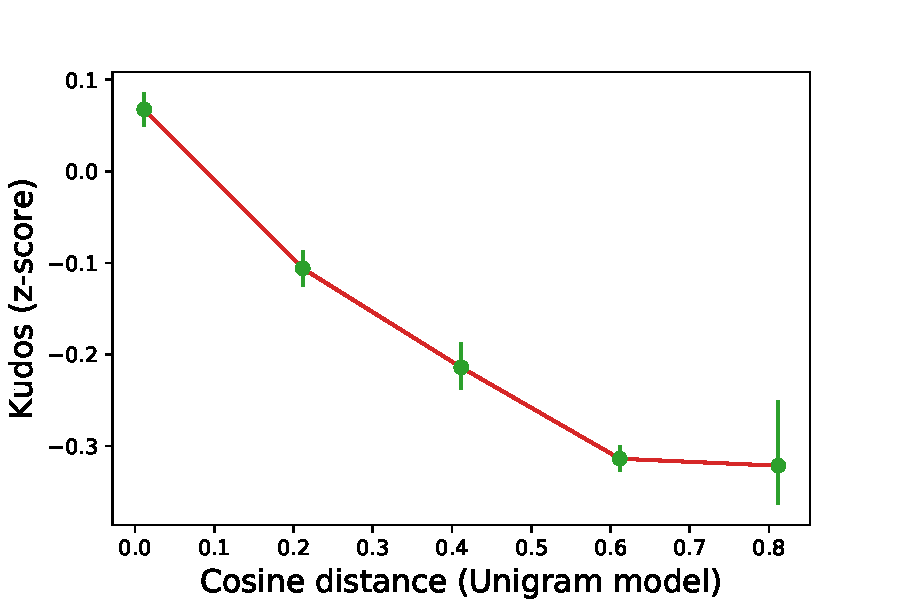
\includegraphics[width=\textwidth]{/unigram_cos_kudos_z_toprev_samplew.pdf}
        \caption{Negative correlation between novelty and Kudos, using the unigram model. As the cosine distance between a fiction and the ``average" of previous fictions increase, the average z-score of Kudos decrease.}
        \label{fig:unigram_cos}
    \end{subfigure}
    ~ %add desired spacing between images, e. g. ~, \quad, \qquad, \hfill etc. 
      %(or a blank line to force the subfigure onto a new line)
    \begin{subfigure}[b]{0.7\textwidth}
        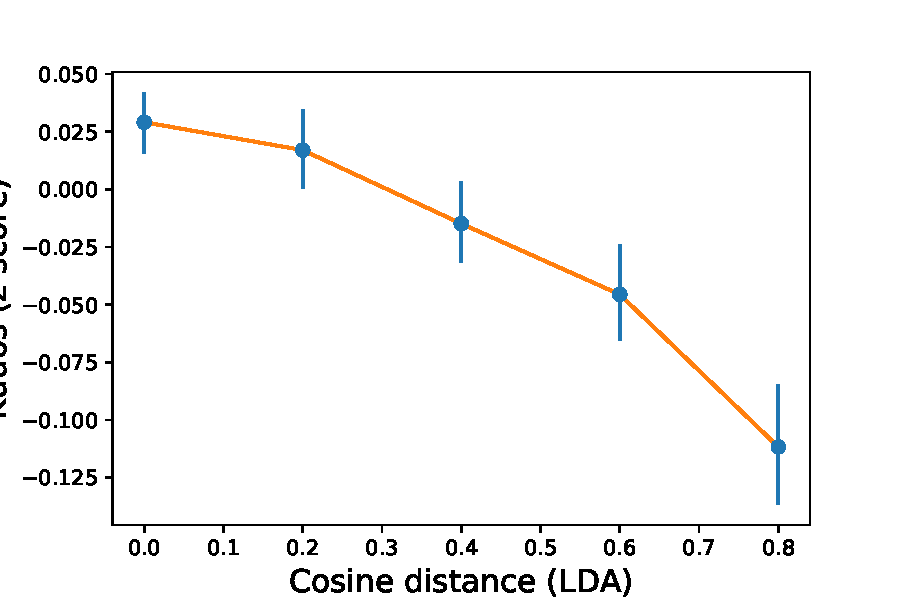
\includegraphics[width=\textwidth]{/lda_cos_kudos_z_toprev.pdf}
        \caption{Negative correlation between novelty and Kudos, using topic modeling. The cosine distance is calculated between the topic distribution of a fiction and the average of topic distribution of previous fictions. As cosine distance increases, the average z-score of Kudos decrease.}
        \label{fig:lda_cos}
    \end{subfigure}
    \caption{Relation between novelty and Kudos on a document level}\label{fig:novelty_kudos_doc}
\end{figure}

\begin{figure}[htbp]
\begin{center}
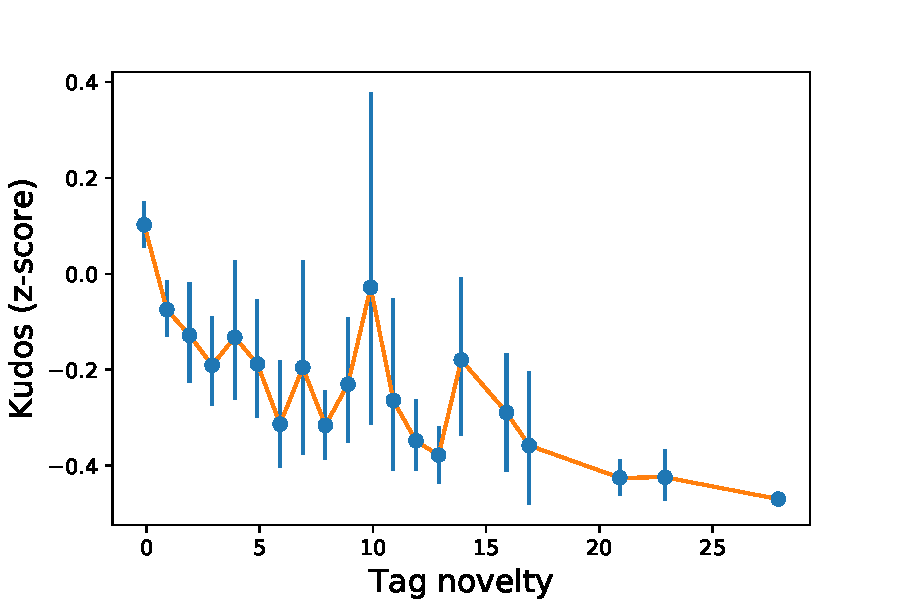
\includegraphics[width=0.7\textwidth]{/tag_novelty_kudos.pdf}
\caption{Tag novelty and Kudos. }
\label{fig:tag_novelty}
\end{center}
\end{figure}

\section*{Discussion}
We have proposed three ways to quantify the novelty of fanfictions. We do this by modeling the texts of the fictions, and using document similarity measurements to calculate the distance between a fiction and the ``average'' fiction of its time and fandom; and also by considering the author-generated tags of the fictions, calculating the ``surprise'' of observing these tags. All methods have presented a negative correlation between a fanfiction's novelty and the Kudos that it receives, indicating that more novelty leads to less hedonic value.

Our results show a pattern diverting from the Wundt-Berlyne curve: instead of a reversed-U shape, we observe the hedonic value consistently decreasing when novelty increases (Fig \ref{fig:unigram_cos}, \ref{fig:lda_cos}, \ref{fig:tag_novelty}). This may be explained by the nature of fan works -- because fans desire to see familiar characters and stories, it is reasonable for them to prefer fanfictions that stay close to the original works. Presumably, a similar psychology may explain the abundance of sequel and spin-off films in today's film market. A possible extension of this work is therefore to investigate if the novelty-Kudos pattern holds for pop culture products other than fanfictions. 


\section*{Methods}

\subsection*{Data collection}
We collected fanfictions from 50 fandoms on AO3, according to its list of most popular fandoms as of March 2016 \footnote{from this list: \url{http://archiveofourown.org/media}}. To avoid duplication, we remove fandoms with heavy overlapping (e.g.: we keep \emph{Marvel} and removed \emph{Marvel movies}). Fandoms that cover diversed topics (e.g.\emph{k-pop}) are also removed. Finally, we only kept the fictions written in English. This leaves us with 904,760 fictions from 25 fandoms. In our analysis, only samples of the data are used. 

Besides the work texts, we also collected metadata including 23 fields. We only used information contained in some of these fields. Table \ref{tab:metadata} gives the names and descriptions of these fields. 

\begin{table}[htp]
\caption{Metadata of the fictions}
\begin{center}
\begin{tabular}[width=0.8\textwidth]{p{2cm}|p{4cm}|p{5cm}}
  \hline			
 Fields & Description & Usage\\ 
   \hline			
Text & The fiction texts. & All text analysis are carried out on these texts.\\\hline
Title & Titles of the fictions. & Used to identify the fictions. \\\hline
Fandoms & Describes which fandom(s) the fiction belongs to. & Used to categorize the fictions.\\\hline
Author & The author of the fiction. & Used for identifying the fictions and for text analysis. \\\hline
% Hits & The number of times a fiction is clicked on. & A metric for evaluating the fiction's popularity. \\\hline
Kudos & The number of ``likes" that the fiction receives. &  Used for evaluating the fiction's success.\\\hline
Publish Date & The date the fiction was published. & Used for temporal analysis.\\\hline

\hline
\end{tabular}
\end{center}
\label{tab:metadata}
\end{table}%

\subsection*{Language model}
We model the fictions with a unigram language model. The Simple Good-Turing smoothing\cite{gales1995good} is applied to improve the model, and to assign non-zero probabilities to previously unseen unigrams. When creating the set of unigrams, we also remove the rare unigrams that appear in less than 5 documents and left out fictions with less than 500 words.


\subsection*{Topic modeling}
The Python library Gensim's LDA \cite{gensimlda} is used to train topic models on our data. We set the number of topics to 40 and use default values for other parameters. 
\subsection*{Computing tag novelty}


\bibliographystyle{acm}
\bibliography{main}

% https://academic.oup.com/chemse/article/24/2/191/312277 familarity & hedonic value of odors
% http://rsos.royalsocietypublishing.org/content/4/7/170433  Significance and popularity in music production



    
\end{document} 
